\section{Experiments}

\begin{figure}[t]
    \centering
    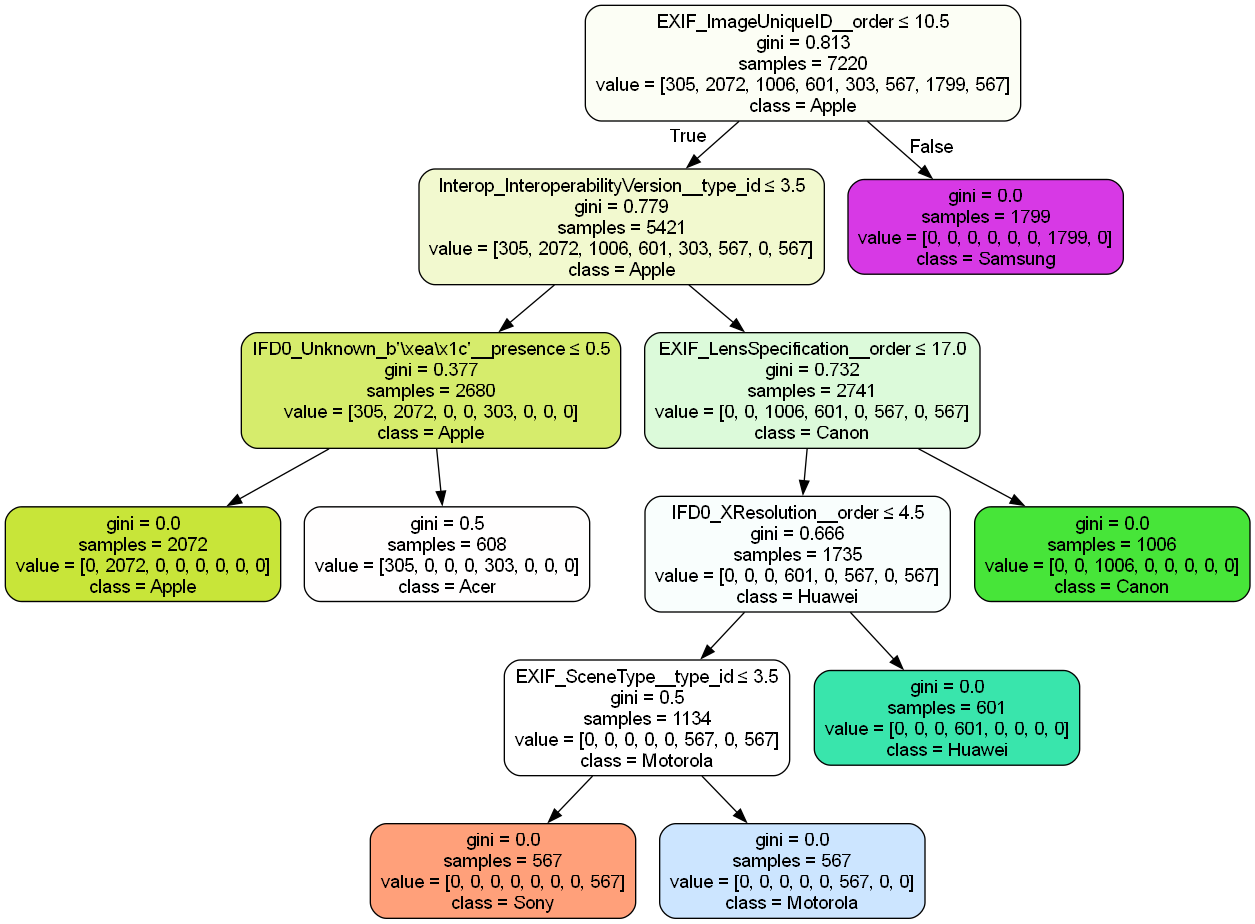
\includegraphics[width=.75\linewidth]{MMM26'//figures/decision_tree_divnoise.png}
    \vspace{-2mm}
    \caption{Decision Tree classifier trained on DivNoise~\cite{casagrande2023divnoise} dataset.}
    \vspace{-5mm}
    \label{fig:decision_tree_divnoise}
\end{figure}

\subsection{Dataset}

\subsubsection{Dresden:}
This is an image database specifically built for the purpose of development and benchmarking of camera-based digital forensic techniques. The dataset comprises 17,242 images from 14 camera manufacturers: Agfa, Canon, Casio, Fujifilm, Kodak, Nikon, Olympus, Panasonic, Pentax, Praktica, Ricoh, Samsung, Sony, and Rollei. All images include complete metadata. For 5 camera makers (Agfa, Canon, Nikon, Pentax, Samsung), there are different camera models. There are 6 camera models under Agfa, 3 under Canon, 3 under Nikon, 2 under Pentax, and 2 under Samsung. Between the camera models, although they are from the same manufacturer, the metadata features are different.

\subsubsection{DivNoise:}
This is a novel dataset designed to support the development of novel source identification techniques. It consists of image and video data from various device cameras, even data acquired from frontal cameras or webcams. This research utilizes 2,249 images from 8 different manufacturers: Acer, Apple, Canon, Huawei, Logitech, Motorola, Samsung, and Sony. For the 2 camera makers (Apple and Samsung), different metadata structures are found.


\subsection{Results}
\subsubsection{Dresden:}
To evaluate model performance, the dataset was split into training and testing sets (80/20) using stratified sampling to preserve class distribution. Two classification models were trained and compared: Random Forest Classifier and Decision Tree Classifier. Both models achieved perfect classification performance, with all predictions matching the ground truth labels. 
This high accuracy is attributed to the rich and distinctive Exif metadata present in the dataset, which provides strong identifying features for each camera \texttt{Make}. The results confirm that camera \texttt{Make} can be reliably inferred using machine learning models trained solely on metadata. To classify up to the camera \texttt{Model}, we create labels by concatenating camera \texttt{Make} and camera \texttt{Model}, such as \textit{Agfa\_DC-504\_0, Canon\_PowerShotA640}. The classification results are visualized in Figure~\ref{fig:dresden_make_model_confusion_matrix}. As shown in the confusion matrix, some camera models are misclassified as they have the same metadata structure as others under the same manufacturer.

\subsubsection{DivNoise:}

To evaluate model performance on the DivNoise dataset, the dataset was split into training and testing sets (80/20) using stratified sampling to maintain class distribution across camera makers.
We trained a Random Forest Classifier and a Decision Tree Classifier, and they have the same classification results. Unlike the Dresden dataset, classification on DivNoise proved to be more challenging. While the model performed well for certain camera makers such as Apple, Canon, Huawei, Motorola, Samsung, and Sony, the overall accuracy was lower since Logitech was misclassified as Acer.
The confusion matrix is shown in Figure~\ref{fig:divnoise_make_random_forest}, which suggests metadata from some devices is less distinctive. The decision tree classifier is visualized in Figure~\ref{fig:decision_tree_divnoise}.
The results of camera \texttt{Model} classification are the same as in Dresden. Typically, some camera models are misclassified as others under the same \texttt{Make} label. Exceptionally, \textit{Logitech\_C920\_Frontal\_0} is always misclassified as \textit{Acer\_AspireE5\_Frontal\_0}.


\subsubsection{Metadata Editing Detection:}
We have discussed the need to demonstrate differences in metadata structure in various scenarios. Table~\ref{tab:metadata_editing_scenarios} describes the changes before and after each scenario.

\begin{table}[t]
\setlength{\tabcolsep}{4pt}
\centering
\caption{Experimental Results for Metadata Editing Detection}
\label{tab:metadata_editing_scenarios}
\begin{tabular}{L{2.5cm}|P{2cm}|p{6.5cm}}
\hline
\textbf{Scenario Type} & \textbf{Case} & \multicolumn{1}{c}{\textbf{Change}} \\
\hline 
\multirow{2}{*}{Social Media} & Facebook & All metadata fields are stripped except \texttt{Artist} and \texttt{Copyright} \\ \cline{2-3}
                              & X & All metadata fields are stripped \\
                              \hline
Metadata Editing Software     & PyExifTool & No changes in structure \\ \hline
Photo Editing Software        & Adobe Photoshop & Many changes in structure (both IFD blocks and fields) \\
\hline
\end{tabular}
\vspace{-3mm}
\end{table}

\section{Demonstration}
The demonstration aims to give users the experience of: (1) observing the decision process of camera \texttt{Make}, camera \texttt{Model} classification using metadata structure, (2) observing the differences/traces in metadata structure when edited or processed by PyExifTool, social media, and Adobe Photoshop. Figure~\ref{fig:demo_extract_view} and figure~\ref{fig:demo_predict_compare} provide screen captures illustrating the system interface and workflow.
Our demo video can be found at \href{https://bit.ly/past_forward}{\small\url{bit.ly/past_forward}}.

\begin{figure}[t]
    \centering
    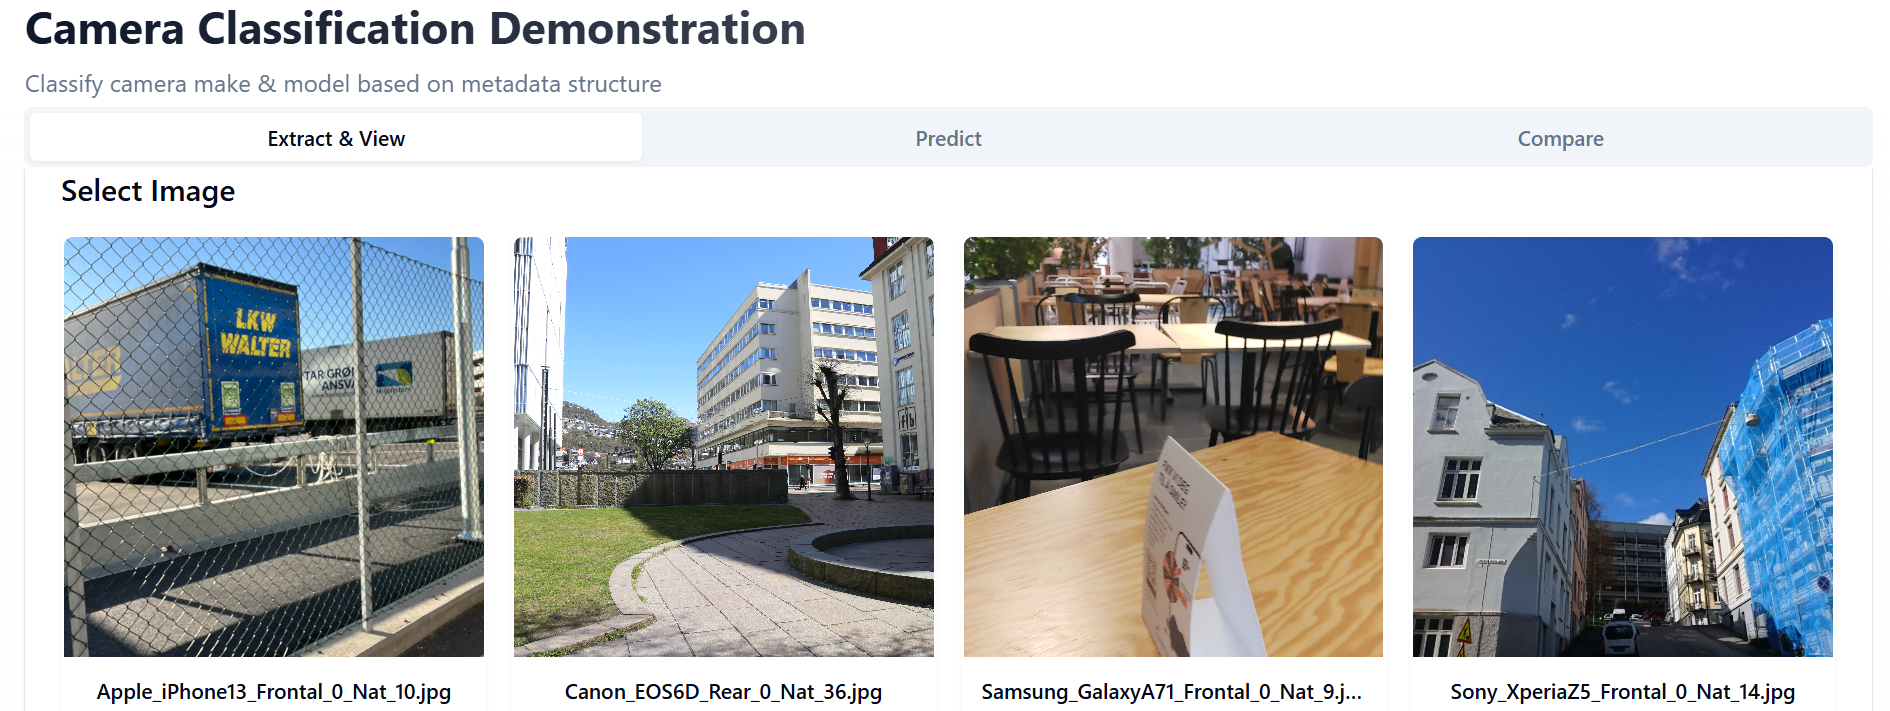
\includegraphics[width=\linewidth]{MMM26'/figures/group_demo_view.png}
    \vspace{-6mm}
    \caption{Extract \& View tab: select image and view metadata structure.}
    \vspace{-3mm}
    \label{fig:demo_extract_view}
\end{figure}

\begin{figure}[t]
    \centering
    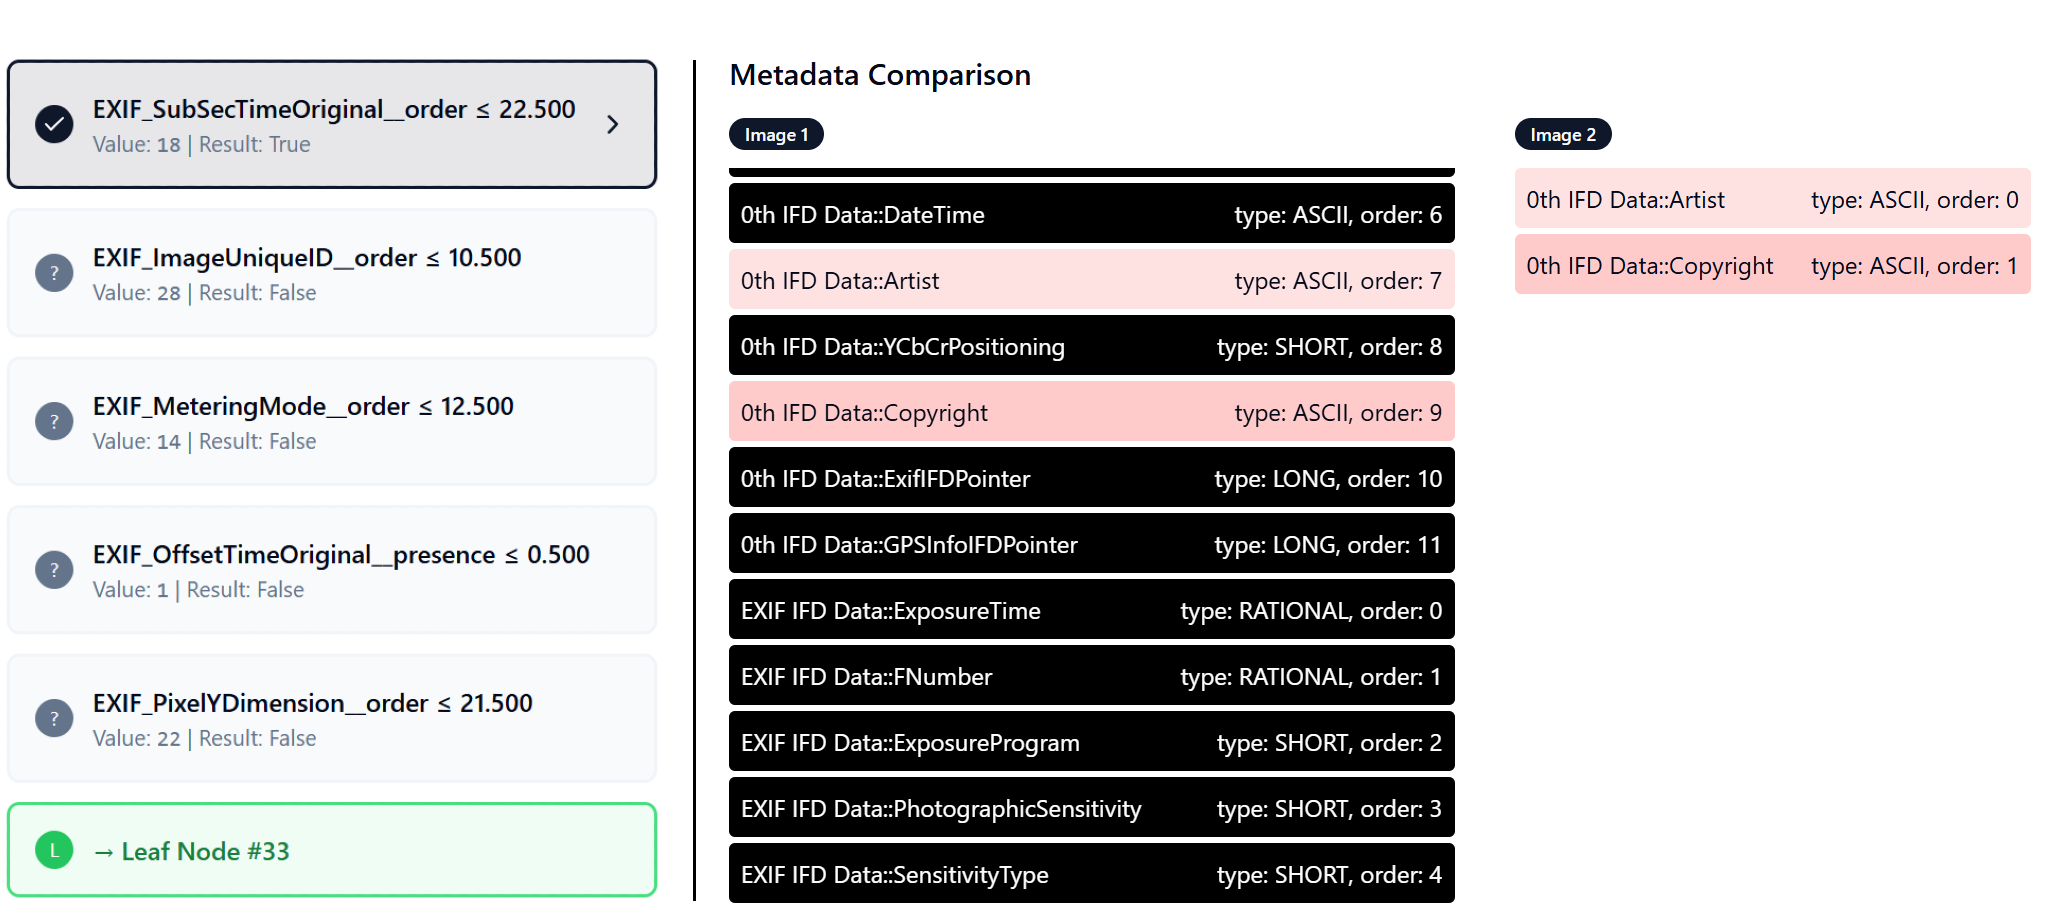
\includegraphics[width=\linewidth]{MMM26'/figures/group_demo_compare.png}
    \vspace{-6mm}
    \caption{Left side: Predict tab: visualize decision process of camera \texttt{Make}/\texttt{Model} prediction. Right side: Compare tab: compare metadata structures between two images.}
    \label{fig:demo_predict_compare}
    \vspace{-2mm}
\end{figure}

